\begin{frame}{Stubmark og efterafgrøder}

\small

\begin{columns}[T]

\begin{column}{0.58\textwidth}

\textbf{Regler for stubmark og efterafgrøder:}

\begin{itemize}[]
\item Efterafgrøde kan være korsblomstrede afgrøder (f.eks. olieræddike, gul sennep, cikorie) eller græs og kornafgrøder
\item Efterafgrøder skal ligge vinteren over til den 20. februar
\item Min. 1 m bred
\end{itemize}

\vspace{0.4em}

\textbf{Gavner arter:}

\footnotesize
Fasan, hare, rådyr, sanglærke, agerhøne, gul vipstjert, rødrygget tornskade, 
gulspurv, agerspurv, gråspurv, markspurv, vild due, vilde bier, humlebier, 
overvintrende insekter, markmus, pindsvin, musvåge, tårnfalk, rødhals

\end{column}

\begin{column}{0.40\textwidth}
\centering
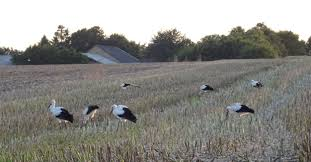
\includegraphics[width=\textwidth]{Billeder/Vildtforvaltning/biotopplantiltag/stubmark.jpeg}
% Bemærk: Jeg ændrede filnavnet til stubmark.jpg – tilpas det til dit faktiske billede
\end{column}

\end{columns}

\end{frame}